%! Author = itgramic
%! Date = 05.12.23

% Preamble
\clearpage
\subsubsection{Skalierung}
\begin{flushleft}
    Datenbanken müssen skalierbar sein.
    Dabei wird unterschieden zwischen einer vertikalen Skalierung (Scale-up) und horizontaler Skalierung (Scale-out).
    Bei der vertikalen Skalierung werden den DB-Servern mehr CPU-Cores und Memory sowie zum Teil Storage hinzugefügt, wobei der Storage in jedem Fall wachsen wird.
    Beim horizontalen Skalieren werden weitere DB-Nodes in den Cluster eingehängt\cite{IZSGZLVT}:
    \begin{figure}[H]
        \centering
        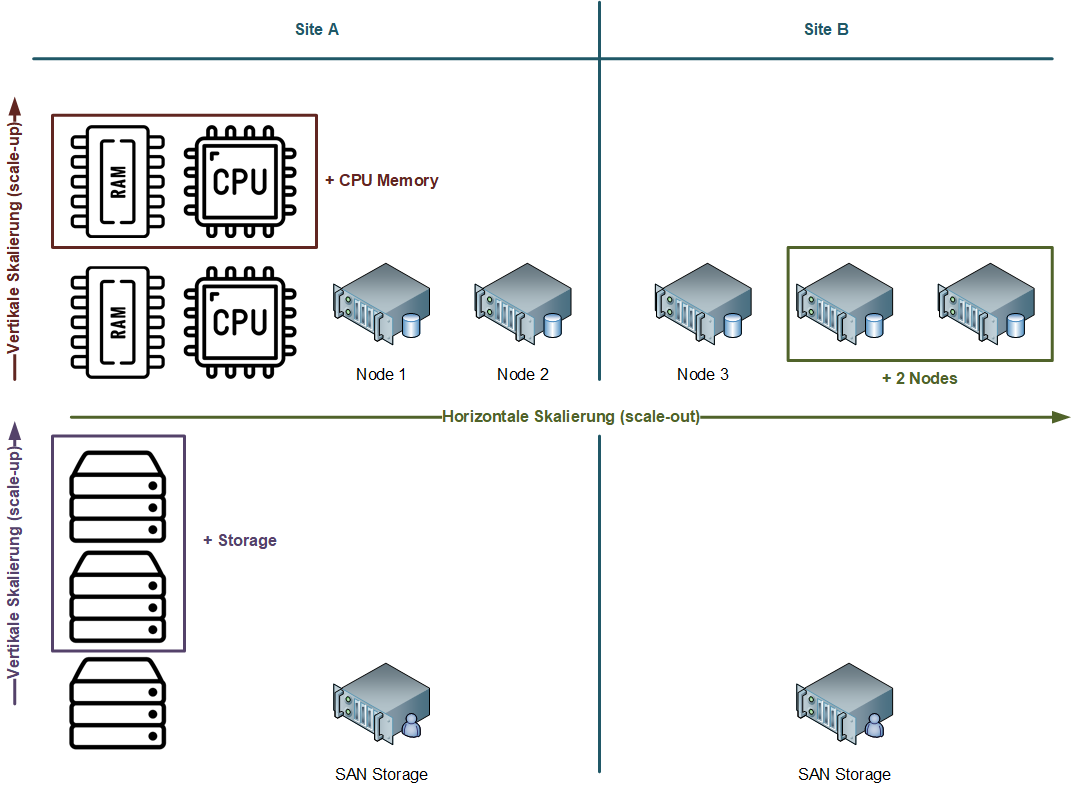
\includegraphics[width=1\linewidth]{source/implementation/evaluation/excursus_architecture/Skalierung}
        \caption{Datenbankskalierung}
        \label{fig:Datenbankskalierung}
    \end{figure}

    Bei monolithischen Datenbanken werden irgendwann die Grenzen der horizontalen Skalierung erreicht und man muss wieder vertikal skalieren, um dem Primary Node genügend Rechnerleistung vorzuhalten.
\end{flushleft}